% Source: M01/S01_SUMMARY.json SHA256 b04416906237b7dfbaf8af5ef8f08b7e9147d10155e495bfcc9a694a5bb691a8.
% Acceptance: scientific_stage2_resume_20261031T205913Z/integration/S01_ACCEPTANCE.json.
% Figures and complete input bindings: temporal/integration/source_bindings.json.
\section{Completed F-continuation recovery}
The earlier incomplete continuation is a historical checkpoint, rather than
the final coverage statement. The authorized Stage~2 recovery filled only
missing statistics: 11 reference histories, 384 null-query histories and two
alternative-query histories, comprising 397 histories and 1,528 procedure
cells. The earlier shorthand of 383 null and three alternative histories is
superseded by this bound input map. All 7,068 originally controlled cells
were preserved. The final bank contains 999 reference statistics, 1,000 null
queries and 150 alternative queries for each of $I_{00},I_{10},I_{01},I_{11}$,
with no unresolved cells. Calibration uses the same add-one rank rule,
including ties through reference statistics greater than or equal to the
query statistic.

\begin{table}[htbp]\centering
\caption{Completed F-continuation rejection counts. All planned queries are
resolved; these proportions replace the historical missingness bounds as
the current numerical checkpoint.}\label{tab:f-stage2-completed}\label{tab:f-continuation}
\begin{tabular}{lrrrr}\toprule
Queries & $I_{00}$ & $I_{10}$ & $I_{01}$ & $I_{11}$\\\midrule
Null ($N=1{,}000$) & 49 (0.049) & 47 (0.047) & 52 (0.052) & 44 (0.044)\\
Alternative ($N=150$) & 150 (1.000) & 122 (0.8133) & 150 (1.000) & 68 (0.4533)\\\bottomrule
\end{tabular}\end{table}

\begin{table}[htbp]\centering
\caption{Completed recovery coverage. Query counts apply to each of the four procedures; repaired and preserved counts refer to procedure cells.}\label{tab:f-recovery-coverage}
\begin{tabular}{lr}\toprule
Quantity & Completed count\\\midrule
Reference histories per procedure & 999\\
Null queries per procedure & 1,000\\
Alternative queries per procedure & 150\\
Preserved procedure cells & 7,068\\
Repaired missing procedure cells & 1,528\\
Profile meshes & 11 of 11\\\bottomrule
\end{tabular}\end{table}

The completed paired interaction
$\overline D=\overline{I^{00}-I^{10}-I^{01}+I^{11}}$ is $-0.006$ under
the null queries (query-unit Monte Carlo standard error $0.00949$), and
$-0.360$ under the alternatives (standard error $0.04564$).
The 2,000 saved resamples in each role and resampling mode are all resolved.
\begin{table}[htbp]\centering
\caption{Completed paired nuisance-interaction means and query-unit Monte Carlo standard errors.}\label{tab:f-completed-interaction}
\begin{tabular}{lrr}\toprule
Queries & Mean $\overline D$ & Monte Carlo SE\\\midrule
Null ($N=1{,}000$) & $-0.006$ & $0.00949$\\
Alternative ($N=150$) & $-0.360$ & $0.04564$\\\bottomrule
\end{tabular}\end{table}
Their descriptive 2.5th, 50th and 97.5th percentiles appear in Table~\ref{tab:f-completed-bootstrap}.

% Completed Stage 2 bootstrap table; historical endpoints retained separately.
\begin{table}[htbp]\centering
\caption{Completed paired-interaction bootstrap summaries. All 2,000 replicates per row are resolved; quantiles are descriptive resampling summaries.}\label{tab:f-completed-bootstrap}
\begin{tabular}{llrrr}\toprule
Queries & Resampling & 2.5th & 50th & 97.5th\\\midrule
Null & Bank only & $-0.022$ & $-0.003$ & $0.015$\\
Null & Bank and paired query & $-0.029$ & $-0.004$ & $0.023$\\
Alternative & Bank only & $-0.4067$ & $-0.3533$ & $-0.3067$\\
Alternative & Bank and paired query & $-0.4667$ & $-0.3600$ & $-0.2533$\\\bottomrule
\end{tabular}\end{table}


These are reference-bank and paired-query resampling sensitivity summaries,
not certified confidence coverage or an independent population calibration.
The null rates are observed simulation frequencies, not proof of nominal
size for every generating law.

\begin{figure}[htbp]\centering
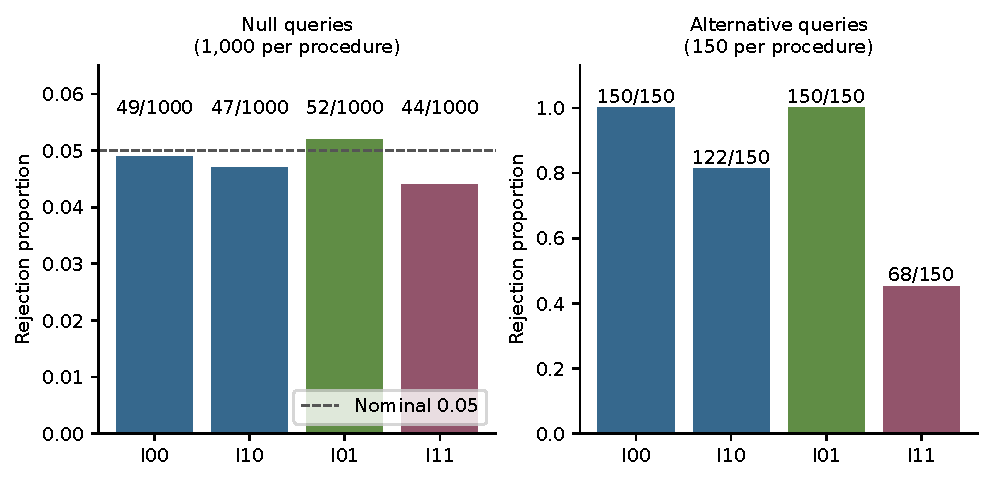
\includegraphics[width=\textwidth]{s01_completed_rejections.pdf}
\caption{Completed planned-denominator F-continuation rejection proportions.
No unresolved outcomes are imputed. The dashed line denotes nominal 0.05.}
\end{figure}



The reference-bank calibration remains an oracle calibration for the
specified synthetic law. It is not a nested fitted-null plug-in calibration:
the proposed 23,760-fit nested bootstrap was excluded by the authorized
scope. Recovery combines original controlled results with an eight-start
compiled procedure only for missing cells, and therefore does not claim
uniform reoptimization of every bank member. Validation comprises 20
resolved-history compatibility controls, independent kernel fixtures and a
three-history raw saved-point pilot, together with complete saved custody
and aggregate arithmetic checks. It does not claim independent raw replay
of every fit or mesh. The finite 195-mode approximation and predictable
pre-event clock convention remain those of the preserved implementation.
